\section{Subdivision Surfaces}
Generalization of spline curves/surfaces. Used for successive refinement (subdivision) and converges to smooth limit surface. \textit{Control Polygon \(\to\) smooth curve}.

\subsection{Line Subdivision}

\begin{definition}[Curve Types]
  \begin{itemize}
    \item \textit{Approximating}: \begin{enumerate}
      \item Split each edge in two
      \item Relocate each (original) vertex with some simple rule.
    \end{enumerate}

    \item \textit{Interpolating}: \begin{enumerate}
      \item Keep old vertices
      \item Generate new vertices by fitting cubic curve to old vertices
      \item \(C^1\) continuous limit curve.
    \end{enumerate}

    \item \textit{Corner Cutting}: \begin{enumerate}
      \item Insert two new vertices at \(1/4, 3/4\).
      \item Remove old vertices and connect the new ones
    \end{enumerate}
  \end{itemize}
\end{definition}

\begin{definition}[Catmull-Clark Filter]
  Approximating equivalent with: insert new point in mid-edge, then filter with \((1/8, 6/8, 1/8)\).
\end{definition}

\subsection{Surface Subdivision}
\begin{tabular}{|c|c|c|c|}
  \hline & \multicolumn{2}{c|}{ Primal } & \multirow{2}{*}{ Dual } \\
  \cline{2-3} & Triangles & Rectangles & \\
  \hline Approx. & Loop & Catmull-Clark & \multirow{2}{*}{\begin{tabular}{c} 
  Doo-Sabin \\
  Midedge
  \end{tabular}} \\
  \hline Interp. & Butterfly & Kobbelt & \\
  \hline
\end{tabular}

\begin{definition}[Primal]
  Faces are split into sub-faces.
\end{definition}

\begin{definition}[Dual]
  Vertices are split into multiple vertices.
\end{definition}

\begin{definition}[Approximating]
  Control points are not interpolated.
\end{definition}

\begin{definition}[Interpolating]
  Control points are interpolated.
\end{definition}

\begin{theorem}
  Different subdivision rules for each valence.
\end{theorem}

\begin{algorithm}[Doo-Sabin]
  Generalization of Bi-quadratic B-Splines.

  \textit{Applied to}: Polygonal meshes

  \textit{Creates}: \(G^1\) -- \(C^0\) for center of irregular polygons after 1 step and \(C^1\) everywhere else.
\end{algorithm}

\begin{algorithm}[Catmull-Clark]
  Generalization of Bi-cubic B-Splines.

  \textit{Applied to}: Polygonal meshes

  \textit{Creates}: \(G^2\) -- \(C^1\) for \(\text{deg}(v) \neq 4\) and \(C^2\) everywhere else.
\end{algorithm}

\begin{algorithm}[Loop]
  Generalization of box-splines.

  \textit{Applied to}: Triangle meshes

  \textit{Creates}: \(G^2\) -- \(C^2\) for \(\text{deg}(v) \neq 6\) and \(C^2\) everywhere else.
\end{algorithm}

\begin{algorithm}[Butterfly Subdivision]
  \textit{Applied to}: Triangle meshes

  \textit{Creates}: \(G^1\) -- \(C^0\) for \(\text{deg}(v) = 3\) or \(> 7\) and \(C^1\) elsewhere.
\end{algorithm}

\begin{theorem}
  Catmull-Clark \& Loop are the best schemes.
\end{theorem}

\begin{itemize*}
  \item Flexible modeling
  \item Scalability
  \item Usability
\end{itemize*}

\makecell{
  \textbf{Start} \\
  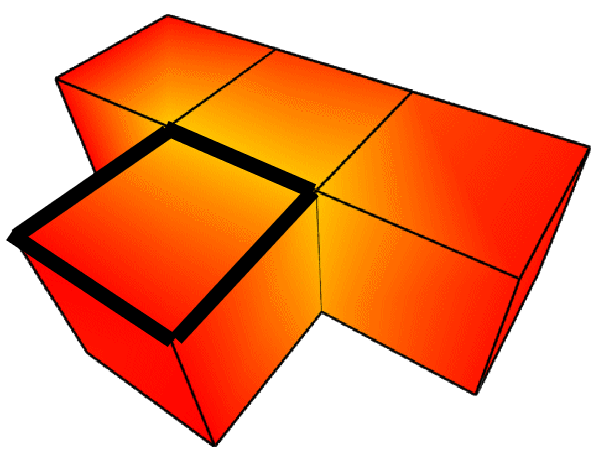
\includegraphics[width=0.3\columnwidth]{assets/start-square.png}
}
\makecell{
  \textbf{Doo-Sabin} \\
  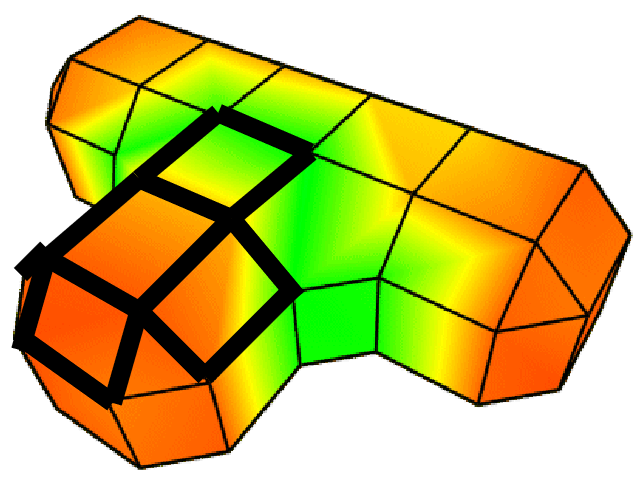
\includegraphics[width=0.3\columnwidth]{assets/doo-sabin.png}
}
\makecell{
  \textbf{Catmull-Clark} \\
  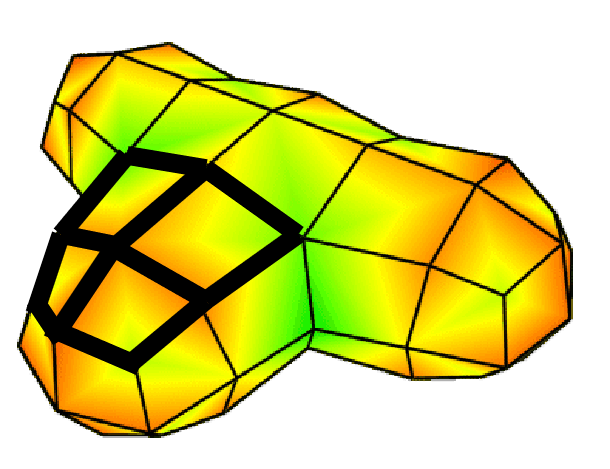
\includegraphics[width=0.3\columnwidth]{assets/catmull-clark.png}
}
\makecell{
  \textbf{Start} \\
  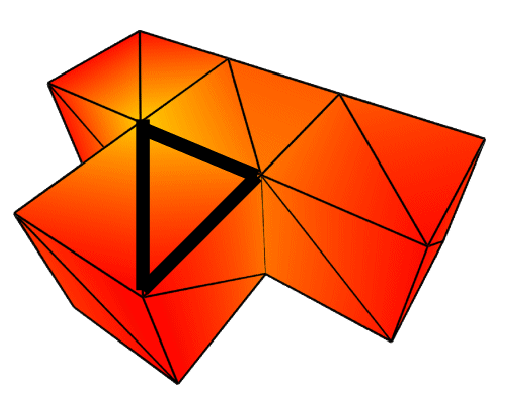
\includegraphics[width=0.3\columnwidth]{assets/start-triangle.png}
}
\makecell{
  \textbf{Loop Subdivision} \\
  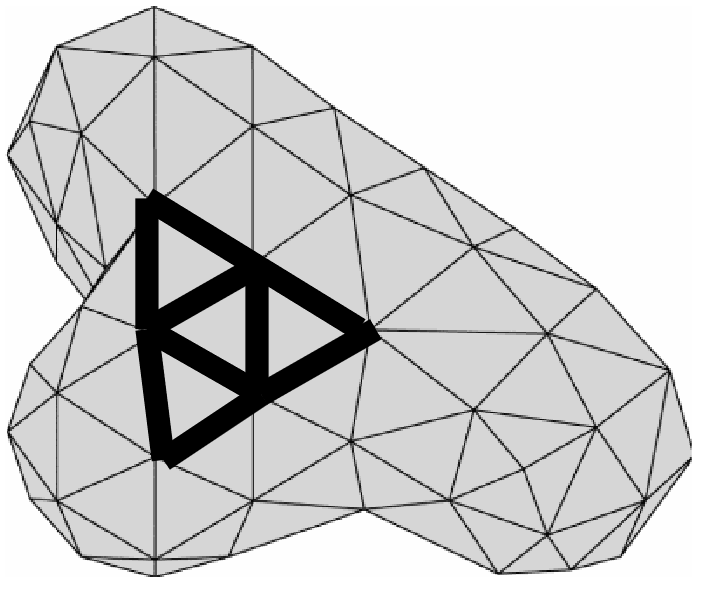
\includegraphics[width=0.3\columnwidth]{assets/loop-subdivision.png}
}
\makecell {
  \textbf{Butterfly} \\
  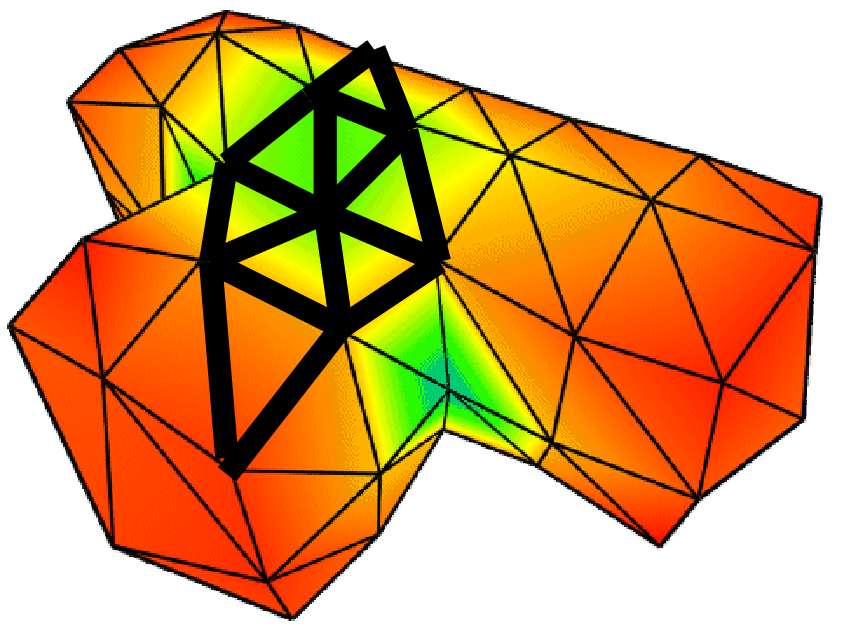
\includegraphics[width=0.3\columnwidth]{assets/butterfly.png}
}